\documentclass[a4paper]{article}

\usepackage[english]{babel}
\usepackage[utf8x]{inputenc}
\usepackage[T1]{fontenc}
\usepackage[a4paper,top=3cm,bottom=2cm,left=3cm,right=3cm,marginparwidth=1.75cm]{geometry}
\usepackage{amsmath}
\usepackage{subcaption}
\usepackage{graphicx}
\usepackage[colorinlistoftodos]{todonotes}
\usepackage[colorlinks=true, allcolors=blue]{hyperref}

\title{Web Technologies: Final}
\author{Charana Nandasena (an15739) and Joshua Van Leeuwen (jv15626, 23305) University of Bristol}

\begin{document}
\maketitle

\section{Prerequisites}
\begin{itemize}
  \item{We are using secure HTTP through use of a self-signed certificate and as
    such, our personal certificate authority must be added to you chosen
    browser. This root CA can be found here `\textit{site/secrets/rootCA.pem}'.}
  \item{We are utilising docker containers in our website to isolate nodejs
    jobs, and although not required, it is recommended that this is installed
    and running. If installed, ensure docker is running by checking the
    systemd unit it running `\textit{systemctl start docker}' on Linux or that the
    `\textit{Docker.app}' process is running on MacOS. Failing this, the server
    will fall back to utilising the local userspace however, this is not the
    intended execution.}
  \item{Once `\textit{server.js}' is running, the server can be reached at
    `\textit{https://localhost:8080}'}
\end{itemize}

\section {Introduction}
This website is designed to be an educational tool for users to learn to program
JavaScript. This is primarily done by users completing a set of JavaScript
programming tasks where their progress is tracked. A supporting forum is
included whereby users are able to create forum `threads' where they are able to
ask questions or have general discussions with the community. Some games are
also included to demonstrate the possibilities of what the user will be able to
create once the user has completed the website tasks and furthered their ability
to code using JavaScript.

Although the user is able to browse the website, much of the functionality
requires the user to have signed up and have an active session. This grants the
user the ability to post and reply on the forum as well as attempt the
challenges.

\section {HTML and CSS - A}

\begin {itemize}
	\item EJS for dyanamic webpages, html templating and generation
    \item webpage XHTML delivery and Ran HTML through XHTML validator jar.
    \item Examples
    	\subitem Figure \ref{fig:login} shows use of css animation keyframes including basic 2D translation and 3D rotations, box shadows for popin/popout affect, absolute positioning with z-index manipulation to manipulate layers etc.
        \subitem Figure \ref{fig:signup_popup} shows use of background color linear gradients, css filters (specifically blur), a popup using html and javascript show/hide handlers  etc.
\end {itemize}

\section{JavaScript}
JOSH - Basic javascript work. Some API calls, calling docker, reading 
writing files, a few simple games.
CHARANA - 

\section{PNG - A}

Two images were made in GIMP as seen in \ref{fig:editor_success} and \ref{editor_failure}.
\ref{fig:sad_background} and \ref{fig:success_background} were used as the backgrounds respectively and \ref{fig:hamster_failed} and \ref{fig:hamster_success} were used as the foregrounds respectively.

The associated images for each graphic were first resized, manipulated (colors edited, portions removed/moved etc.) and background thresholded from foreground before being replaced by an alpha channel.

The cleaned imaged were then imported as individual layers.

A new text layer was created to write the "success" or "wrong", a blur filter subsequently then applied to a duplicate layer obtain the 3D text affect.
A gradient color was created and applied to the original text layer (only coloring the front facing side of the text).

The layers were then combined and exported as a PNG.
This was done for each image.

\begin{figure}[h!]
  \centering
  \begin{subfigure}[b]{0.3\linewidth}
    
\includegraphics[width=\linewidth]{png-creation/hamster-failed.png}
    \caption{Hamster Failed}
    \label{fig:hamster_failed}
  \end{subfigure}
  \begin{subfigure}[b]{0.3\linewidth}
    
\includegraphics[width=\linewidth]{png-creation/sad-background.png}
    \caption{Sad Background}
    \label{fig:sad_background}
   \end{subfigure}
   \begin{subfigure}[b]{0.3\linewidth}
    
\includegraphics[width=\linewidth]{png-creation/wrong-graphic.png}
    \caption{Wrong Graphic}
    \label{fig:wrong_graphic}
  \end{subfigure}
  \caption{}
\end{figure}
\begin{figure}[h!]
  \centering
  \begin{subfigure}[b]{0.25\linewidth}
    
\includegraphics[width=\linewidth]{png-creation/hamster-success.png}
    \caption{Hamster Success}
    \label{fig:hamster_success}
  \end{subfigure}
  \begin{subfigure}[b]{0.3\linewidth}
    
\includegraphics[width=\linewidth]{png-creation/success-background.png}
    \caption{Success Background}
    \label{fig:success_background}
   \end{subfigure}
   \begin{subfigure}[b]{0.3\linewidth}
    
\includegraphics[width=\linewidth]{png-creation/success-graphic.png}
    \caption{Correct Graphic}
    \label{fig:correct_graphic}
  \end{subfigure}
  \caption{}
\end{figure}

\section{SVG - A}
\ref{fig:logo} is our site logo made in Inkscape.
In creating each component of the logo circles, rectangles and polygons were first draw, these shapes were then converted into paths using the "stroke to path" tool. In creating more complex shapes the "bezier curve" tool was used.
The "edit paths by node" was used to manipulate the curve trajectories,
carefully inserting/removing nodes along the outline to obtain the desired shape. 
Several individual components were then grouped together and flipped horizontally to obtain a symmetrical look.
A linear gradient was finally applied along the vertical axis.

\section{Server - A}
The server has been expanded upon from the original server.js file given.

\begin{itemize}
  \item{Use of URL validation and redirection.}
  \item{Sign up and reply/post field validation.}
  \item{Handling various user data including text, code and images.}
  \item{Generation and validation of captcha to prevent malicious botting of
    sign up requests as well as user submitted forum posts and replies.}
  \item{Extensive use of our own written modules with both private and public exposed
    functions providing APIs to applications of the server.}
  \item{Use of a standard page delivery flow in conjunction with our modules to
    provide server with ease of extensibility. This is achieved through use of
    so called `pre functions' and main data delivery functions that allow
    dynamic data delivery to the EJS HTML template library resulting in
    dynamic pages based on the state of the server and database.}
  \item{Providing HTTPS connection to ensure a secure connection. This is using
    a self-signed certificate which is enabled as described in the perquisites.}
  \item{Use of internally generated and managed cookies to provide user
    sessions.}
  \item{Passwords stored using a salted hash preventing storing passwords as
    plain text in the database.}
  \item{In order to isolate code given by the client, the use of docker
    containers have been used to execute the code, preventing malicious code being
    run in the server namespace. The code will be run in a docker container
    whereby it's stdout/err will be captured and saved to file. This file is
    copied out of the container and is checked against the relevant solution
    file. As described in the perquisites, the use of the local userspace will
    be used instead, in the event of the docker image failing to build, preventing this
    feature.}
\end{itemize}

\section{Database - A}
The SQLite relational database has been used as our database.

\begin{itemize}
  \item{A number of tables are used to store user data, user voting data,
      user challenge progress data, challenge data as well as forum data.}
  \item{Each group of associated tables are accessed by through use of separate
    modules, acting as APIs, all in turn interacting with the main database\_api
    module that manipulates data in the database.}
  \item{Tables are created relational so to provide extensibility to data such
    as the forum replies table relating the forum post table.}
  \item{Passwords are stored as a salted hash along with the salt in the users
    tables to prevent storing as plain text.}
  \item{Modular tables have been used in an effort to reduce read and write
    access of the database.}
\end{itemize}

\section{Dynamic Pages - A}
\begin{itemize}
  \item{Use of the EJS templating framework to build HTML pages based upon
    delivery data from the server.}
  \item{Delivery data is made from database query data as well as non sensitive
    user data based on the session.}
  \item{The use of Asynchronous JavaScript + XML (AJAX) to create dynamic
    changes to the web page}
\end{itemize}

\section{Depth - X}

\appendix

\section{Images}

\begin{figure}[h!]
  \centering
  
\includegraphics[width=1\linewidth]{images/header.png}
  \caption{Header}
  \label{fig:header}
\end{figure}

\begin{figure}[h!]
  \centering
  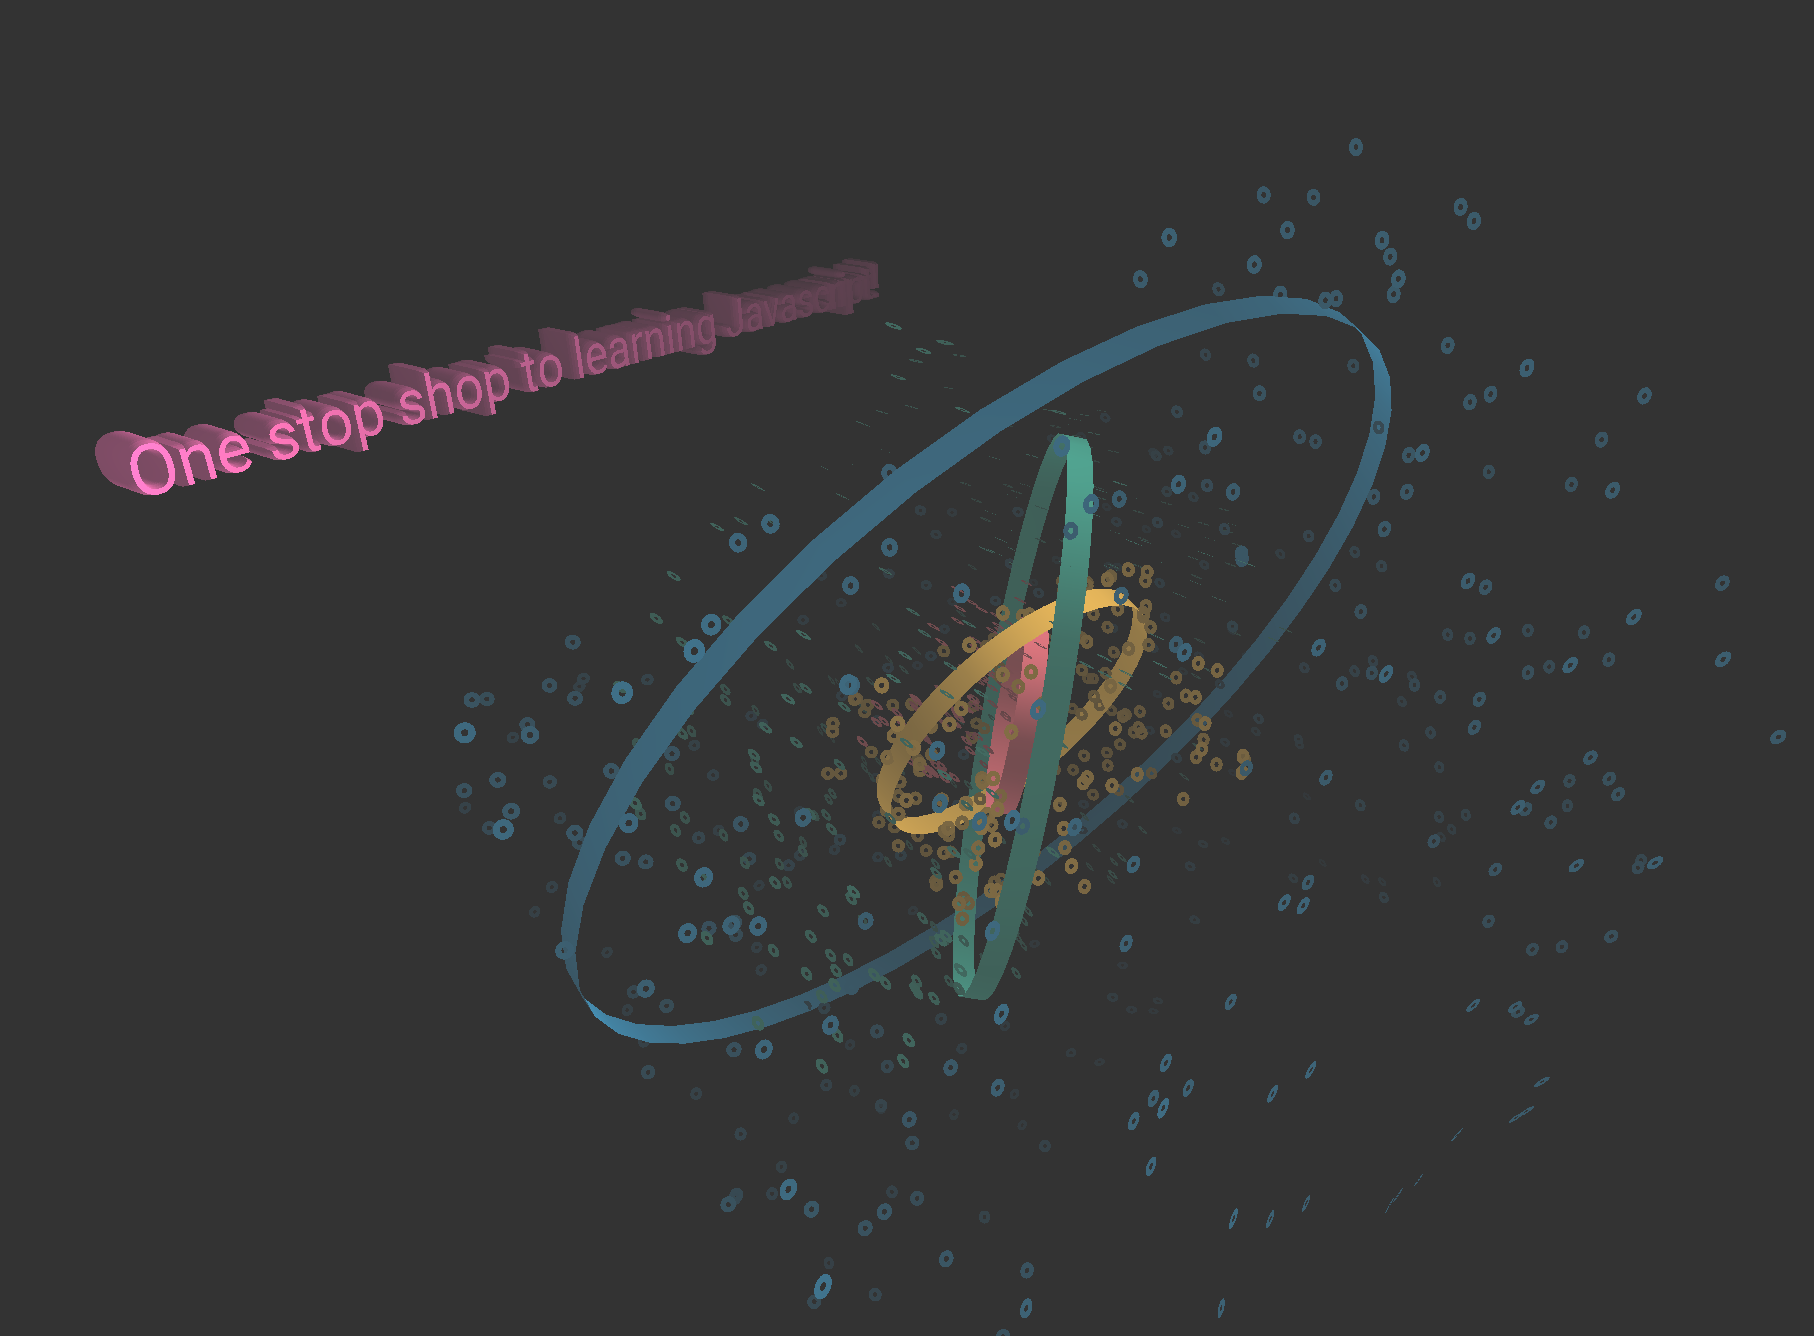
\includegraphics[width=0.75\linewidth]{images/3d_background.png}
  \caption{3D Background}
  \label{fig:3d_background}
\end{figure}

\begin{figure}[h!]
  \centering
  \begin{subfigure}[b]{0.3\linewidth}
    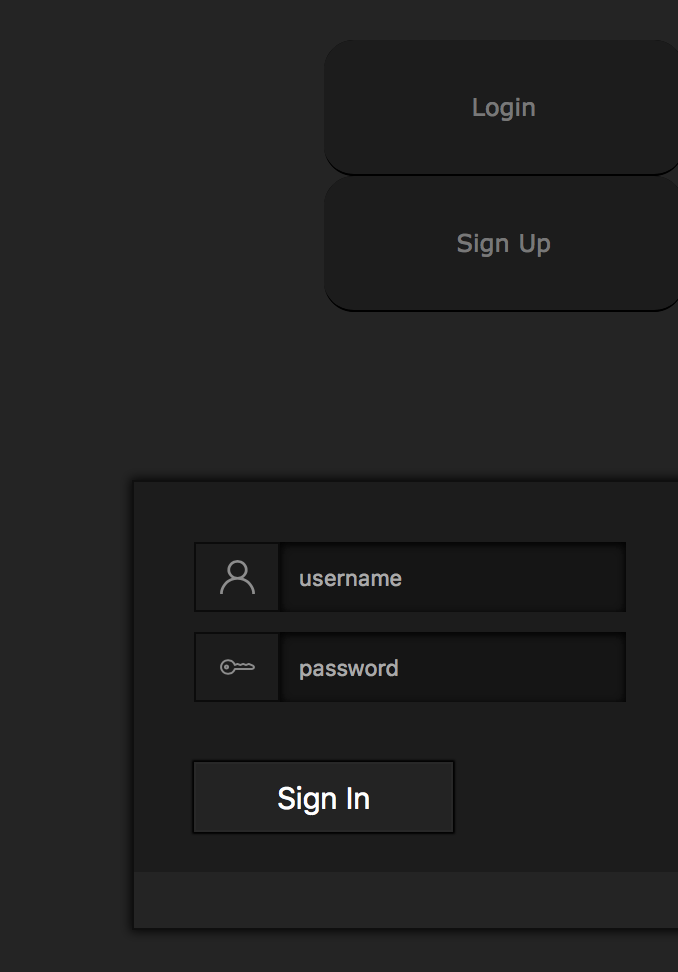
\includegraphics[width=\linewidth]{images/login.png}
    \caption{Settings Popup and Login}
    \label{fig:login}
  \end{subfigure}
   \begin{subfigure}[b]{0.3\linewidth}
    
\includegraphics[width=\linewidth]{images/logo.png}
    \caption{SVG Logo}
    \label{fig:logo}
  \end{subfigure}
   \begin{subfigure}[b]{0.3\linewidth}
    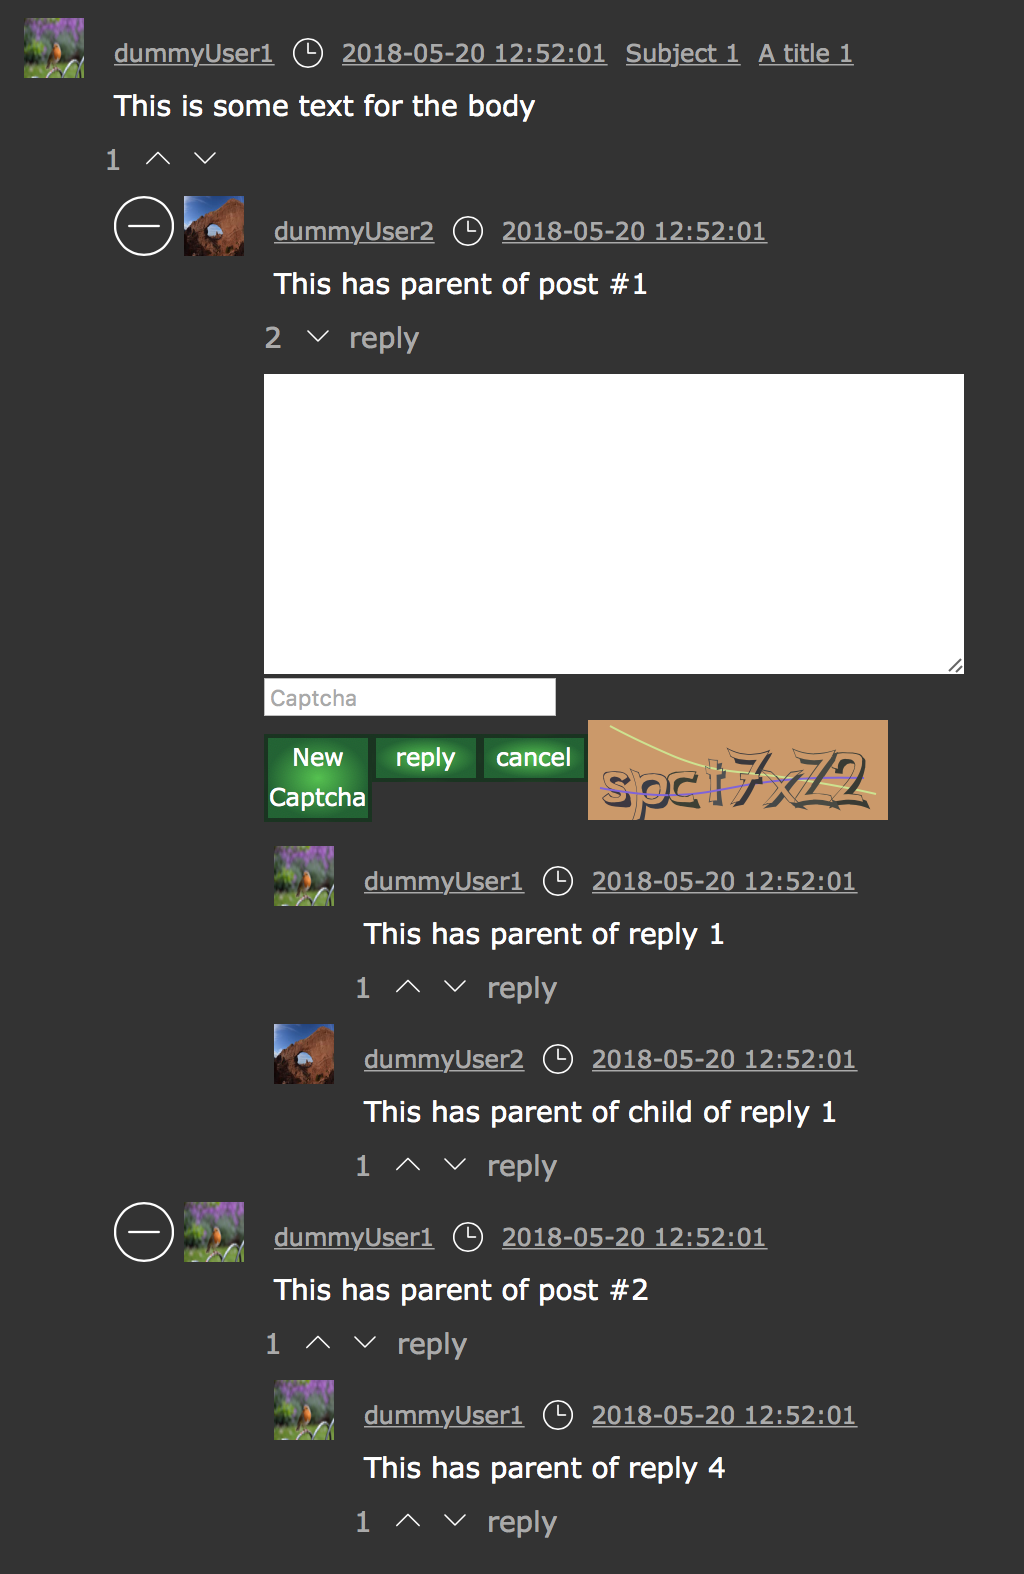
\includegraphics[width=\linewidth]{images/forum-posts.png}
    \caption{Forum Post}
    \label{fig:forum_post}
  \end{subfigure}
  \caption{}
\end{figure}

\begin{figure}[h!]
  \centering
  \begin{subfigure}[b]{0.45\linewidth}
    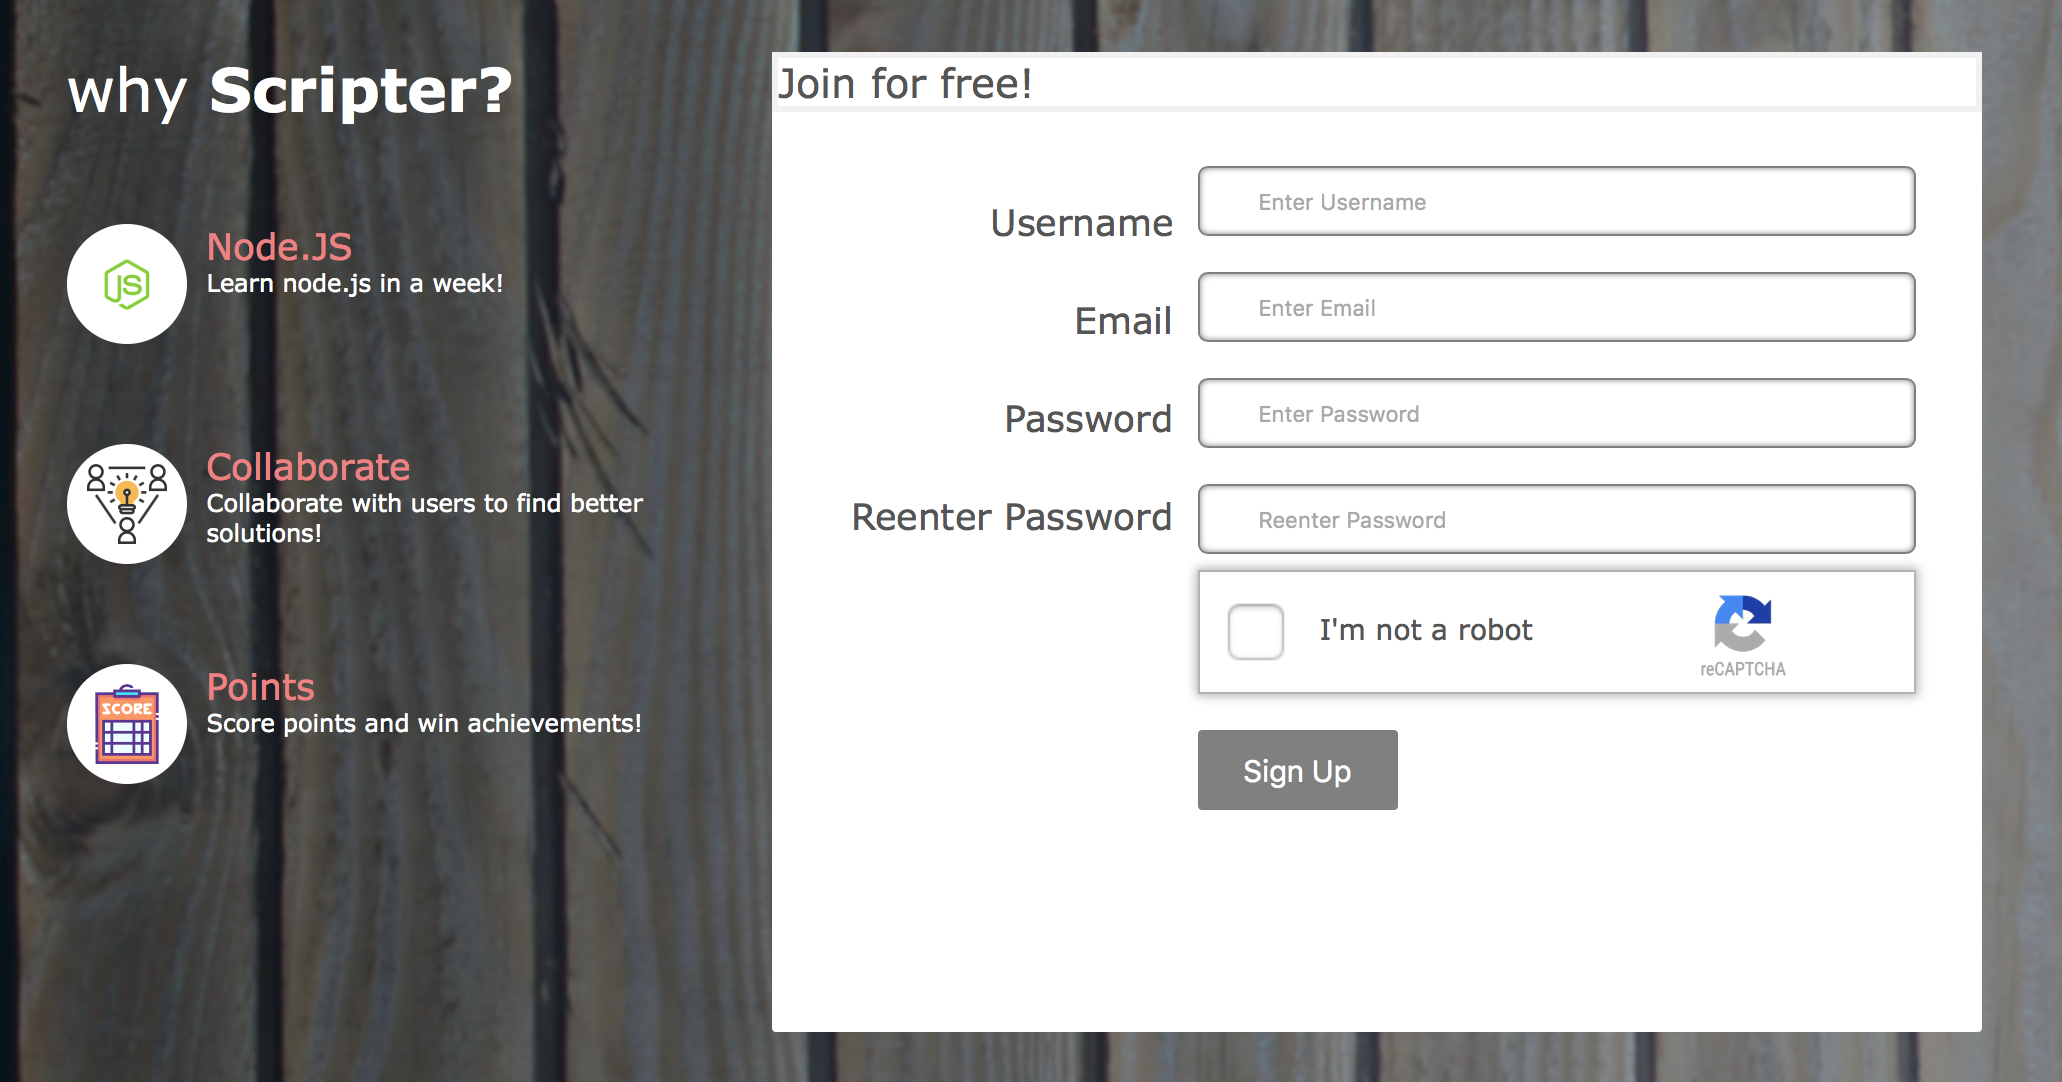
\includegraphics[width=\linewidth]{images/signup-default.png}
    \caption{Sign-Up Default}
    \label{fig:signup_default}
  \end{subfigure}
    \begin{subfigure}[b]{0.45\linewidth}
    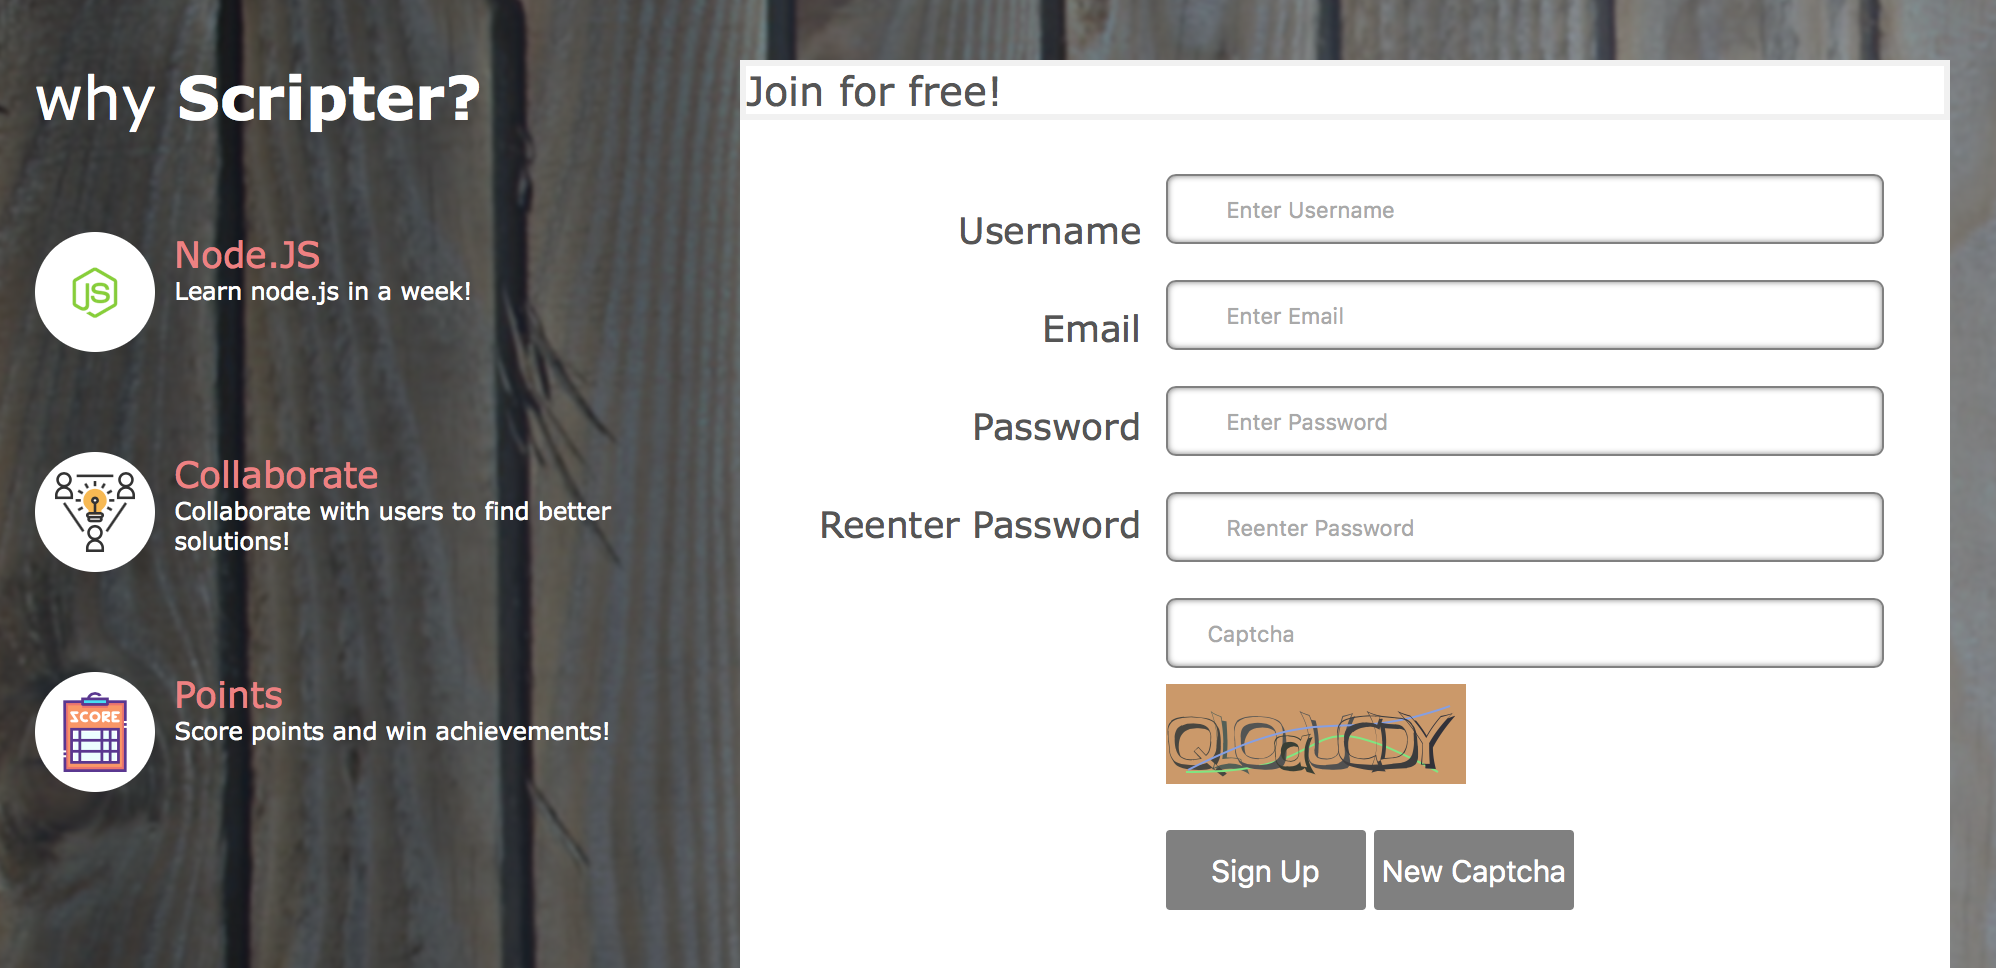
\includegraphics[width=\linewidth]{images/signup-captcha.png}
    \caption{Sign-Up RE-CAPTCHA Popup}
    \label{fig:signup_popup}
  \end{subfigure}
  \caption{}
\end{figure}

\begin{figure}[h!]
  \centering
  \begin{subfigure}[b]{0.3\linewidth}
    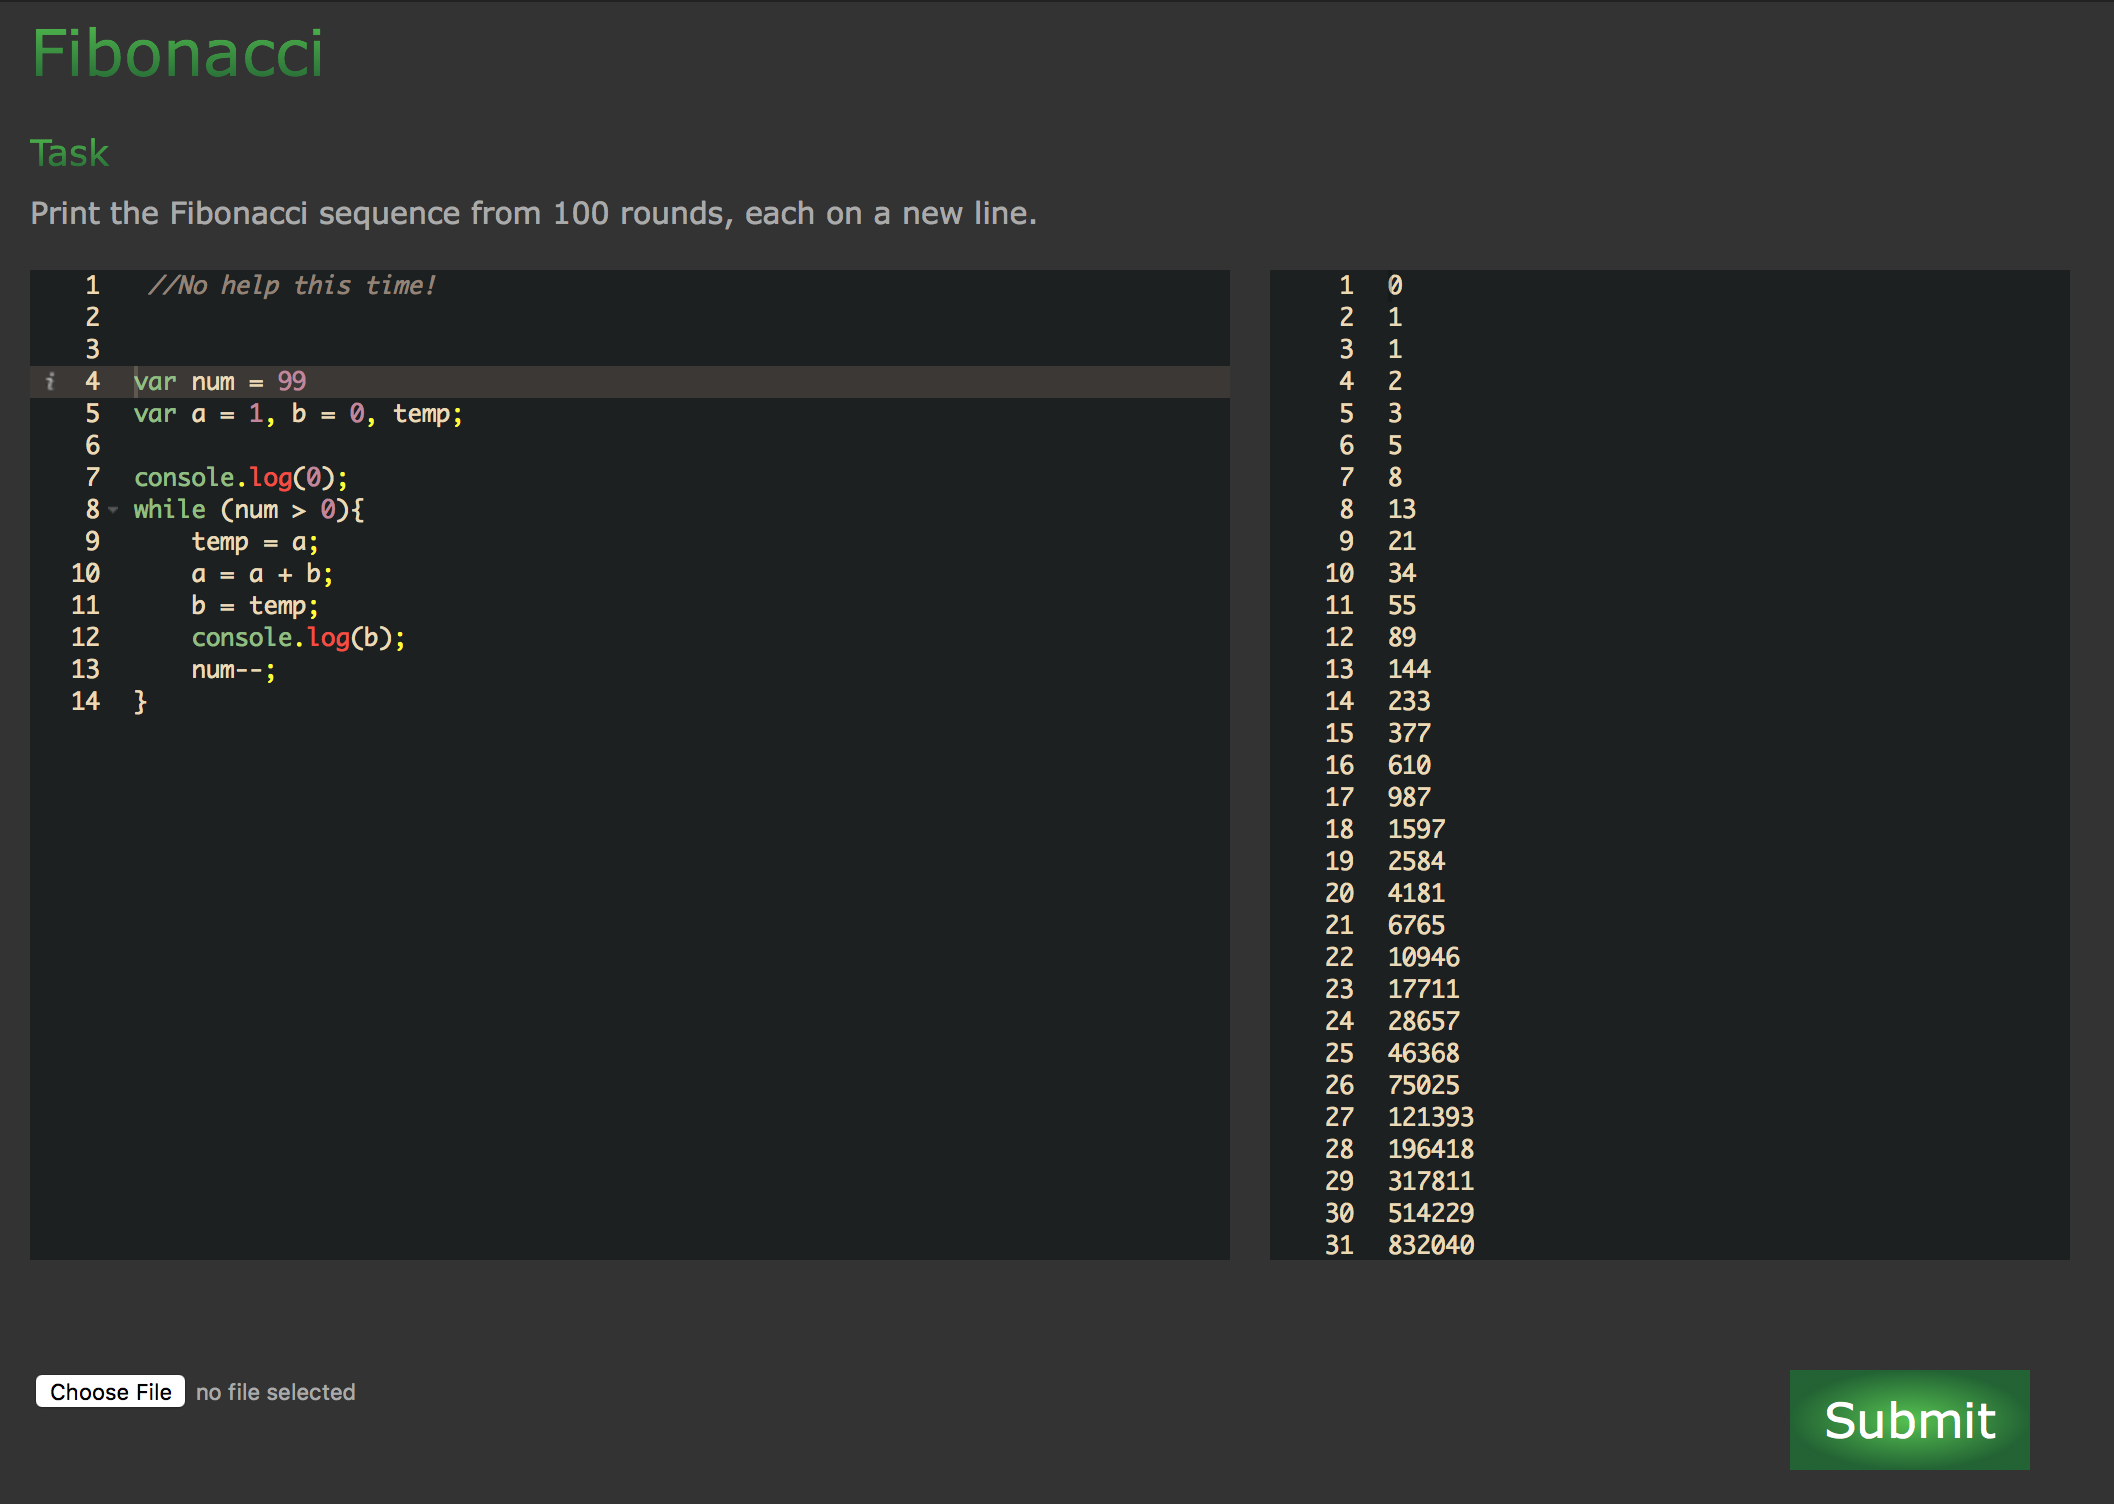
\includegraphics[width=\linewidth]{images/editor-default.png}
    \caption{Editor Default}
    \label{fig:editor_default}
  \end{subfigure}
  \begin{subfigure}[b]{0.3\linewidth}
    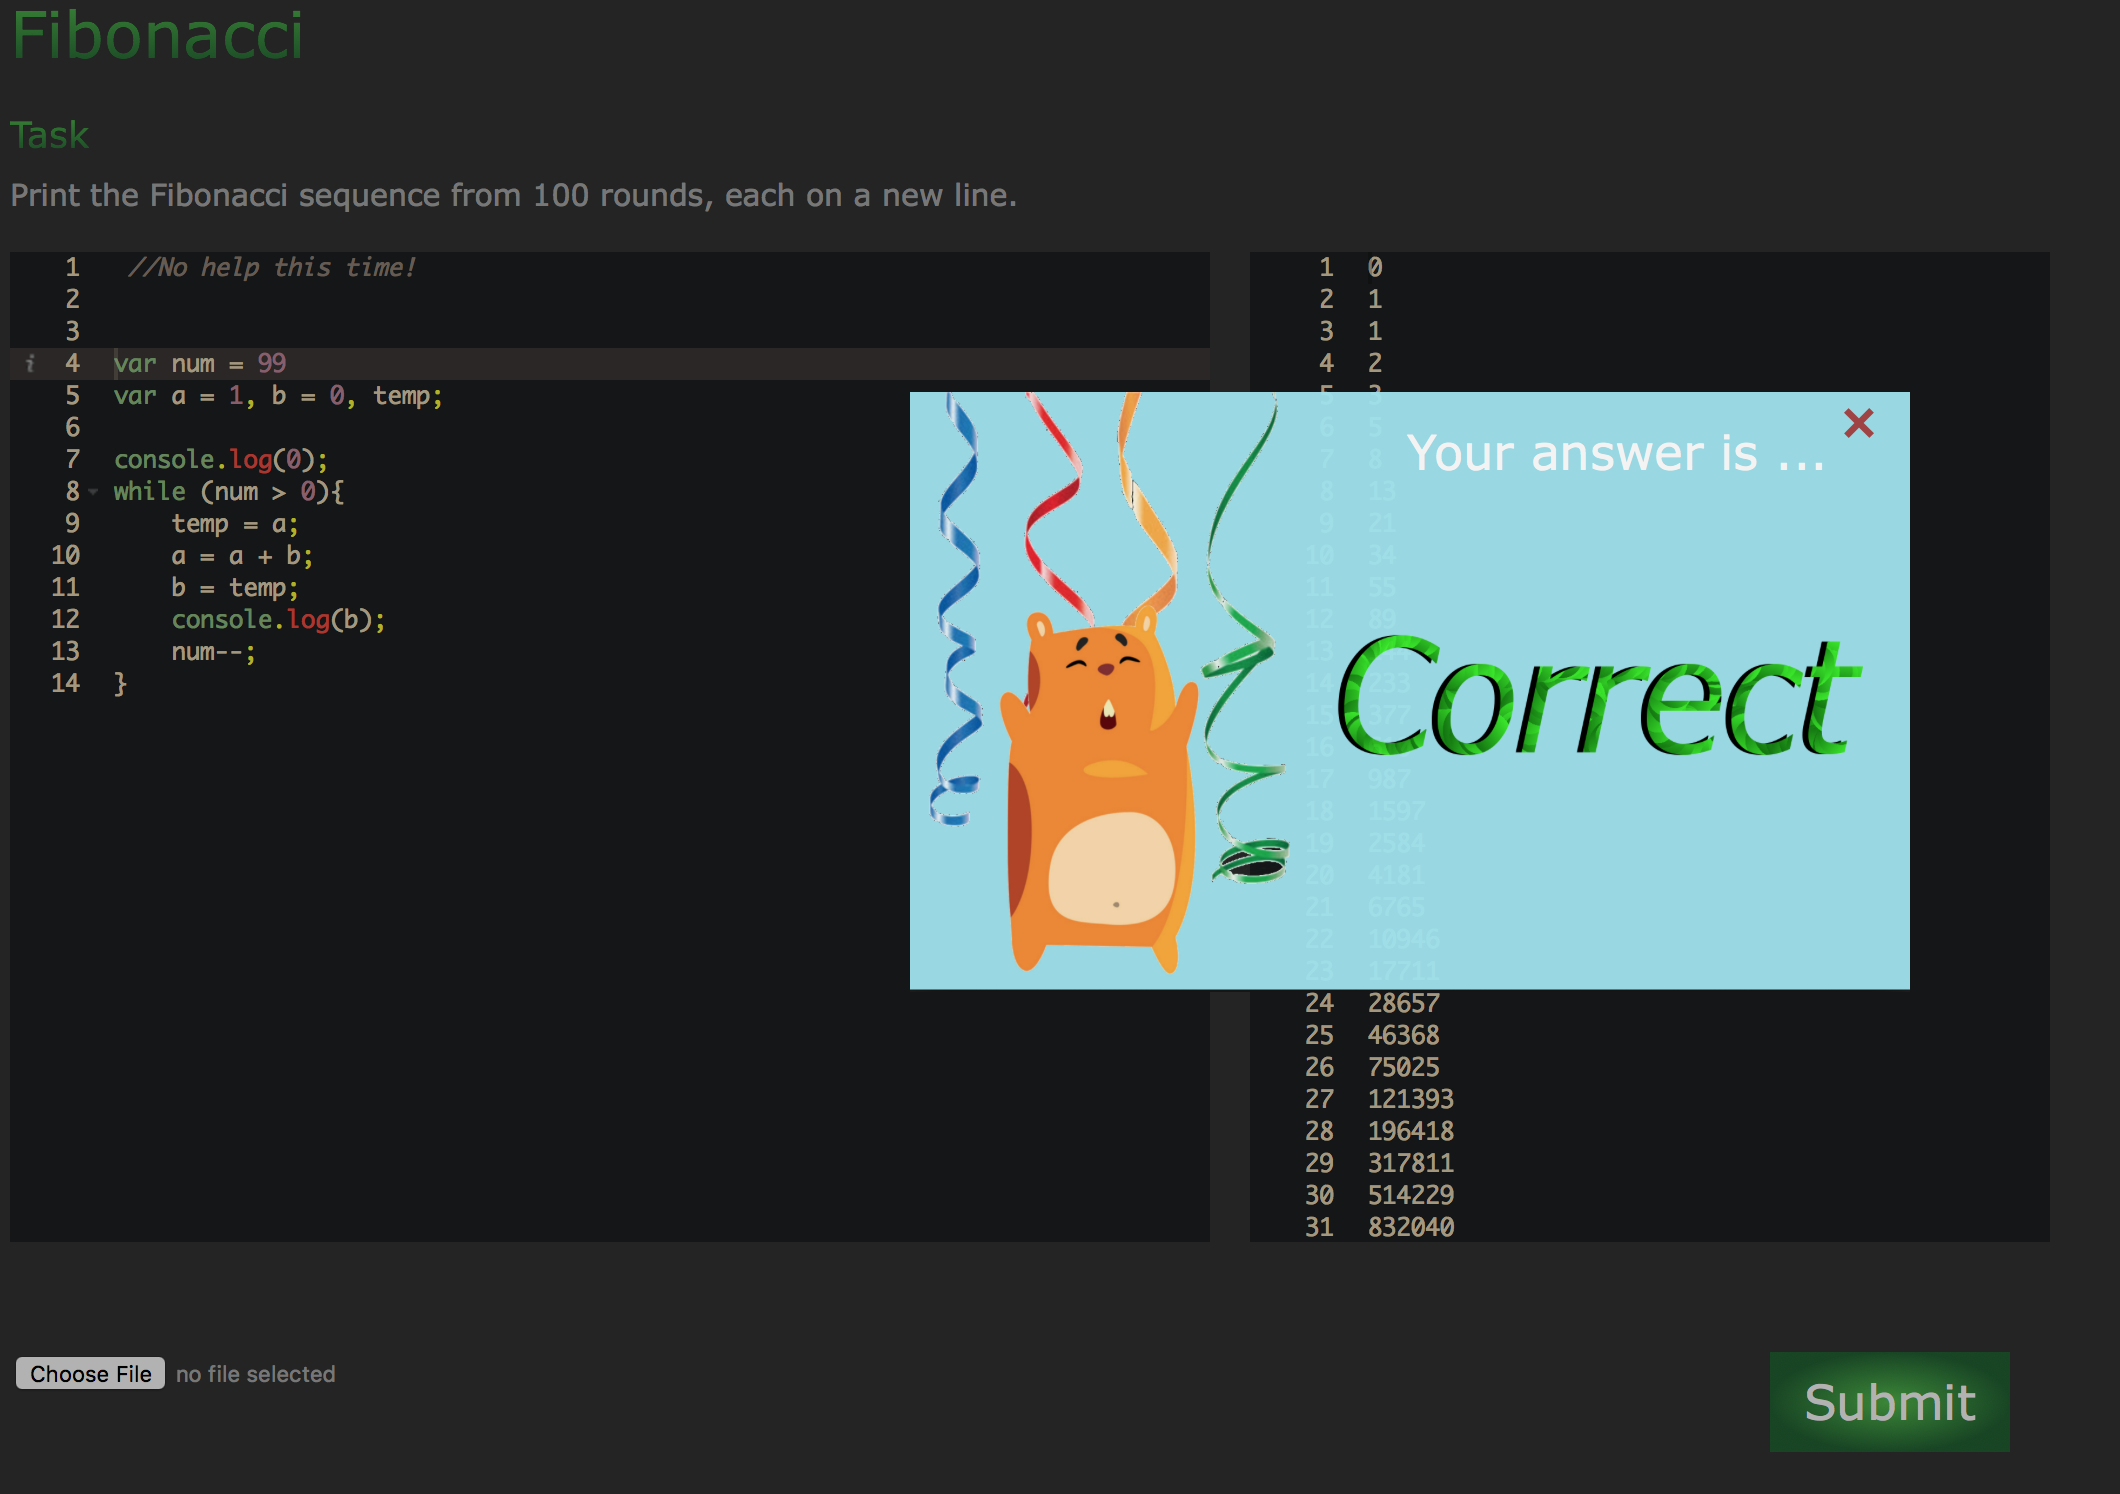
\includegraphics[width=\linewidth]{images/editor-success.png}
    \caption{Editor Success}
    \label{fig:editor_success}
   \end{subfigure}
   \begin{subfigure}[b]{0.3\linewidth}
    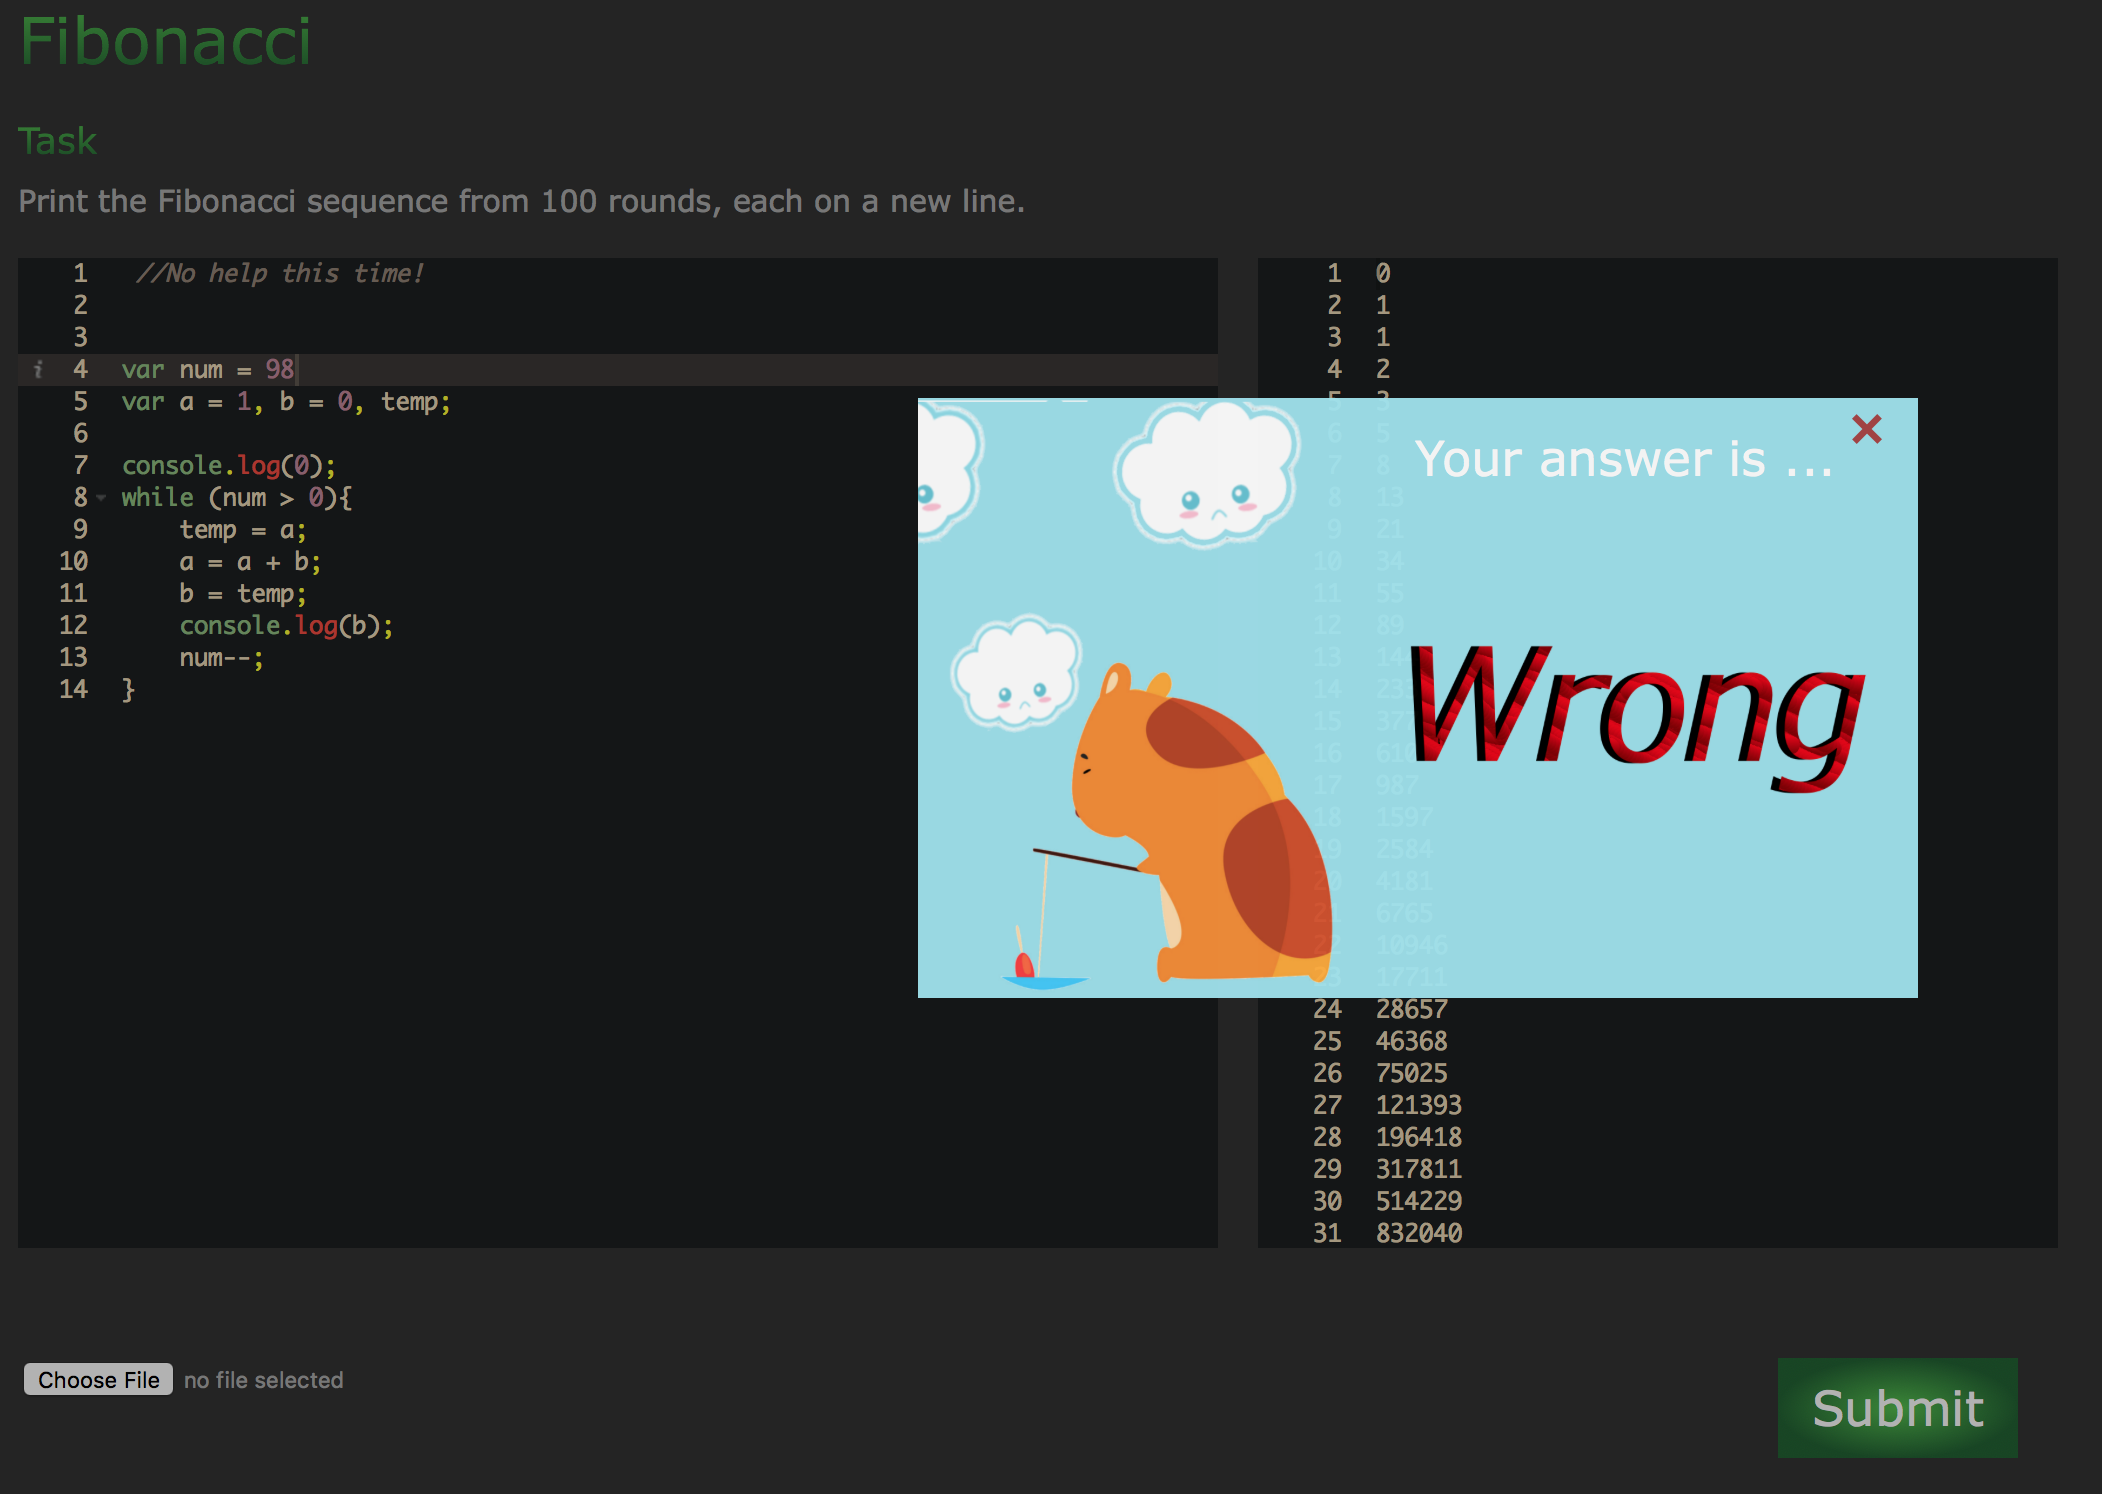
\includegraphics[width=\linewidth]{images/editor-failure.png}
    \caption{Editor Failure}
    \label{fig:editor_failure}
  \end{subfigure}
  \caption{}
\end{figure}

\begin{figure}[h!]
  \centering
  \begin{subfigure}[b]{0.3\linewidth}
    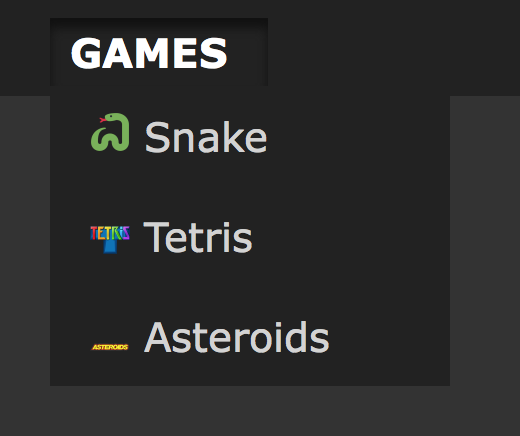
\includegraphics[width=\linewidth]{images/games-dropdown.png}
    \caption{Games Dropdown}
    \label{fig:signup_default}
  \end{subfigure}
  \begin{subfigure}[b]{0.3\linewidth}
    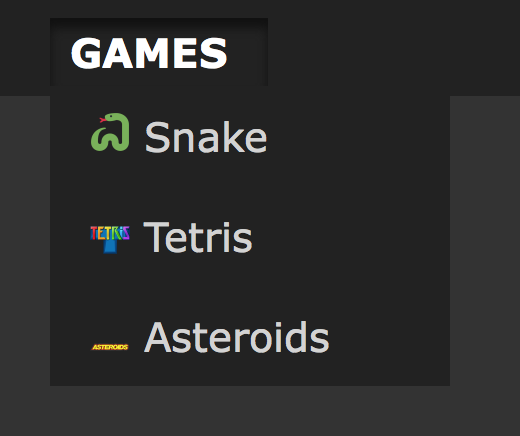
\includegraphics[width=\linewidth]{images/games-dropdown.png}
    \caption{Games Dropdown}
    \label{fig:signup_default}
  \end{subfigure}
  \caption{}
\end{figure}

\end{document}
